\documentclass[1p]{elsarticle_modified}
%\bibliographystyle{elsarticle-num}

%\usepackage[colorlinks]{hyperref}
%\usepackage{abbrmath_seonhwa} %\Abb, \Ascr, \Acal ,\Abf, \Afrak
\usepackage{amsfonts}
\usepackage{amssymb}
\usepackage{amsmath}
\usepackage{amsthm}
\usepackage{scalefnt}
\usepackage{amsbsy}
\usepackage{kotex}
\usepackage{caption}
\usepackage{subfig}
\usepackage{color}
\usepackage{graphicx}
\usepackage{xcolor} %% white, black, red, green, blue, cyan, magenta, yellow
\usepackage{float}
\usepackage{setspace}
\usepackage{hyperref}

\usepackage{tikz}
\usetikzlibrary{arrows}

\usepackage{multirow}
\usepackage{array} % fixed length table
\usepackage{hhline}

%%%%%%%%%%%%%%%%%%%%%
\makeatletter
\renewcommand*\env@matrix[1][\arraystretch]{%
	\edef\arraystretch{#1}%
	\hskip -\arraycolsep
	\let\@ifnextchar\new@ifnextchar
	\array{*\c@MaxMatrixCols c}}
\makeatother %https://tex.stackexchange.com/questions/14071/how-can-i-increase-the-line-spacing-in-a-matrix
%%%%%%%%%%%%%%%

\usepackage[normalem]{ulem}

\newcommand{\msout}[1]{\ifmmode\text{\sout{\ensuremath{#1}}}\else\sout{#1}\fi}
%SOURCE: \msout is \stkout macro in https://tex.stackexchange.com/questions/20609/strikeout-in-math-mode

\newcommand{\cancel}[1]{
	\ifmmode
	{\color{red}\msout{#1}}
	\else
	{\color{red}\sout{#1}}
	\fi
}

\newcommand{\add}[1]{
	{\color{blue}\uwave{#1}}
}

\newcommand{\replace}[2]{
	\ifmmode
	{\color{red}\msout{#1}}{\color{blue}\uwave{#2}}
	\else
	{\color{red}\sout{#1}}{\color{blue}\uwave{#2}}
	\fi
}

\newcommand{\Sol}{\mathcal{S}} %segment
\newcommand{\D}{D} %diagram
\newcommand{\A}{\mathcal{A}} %arc


%%%%%%%%%%%%%%%%%%%%%%%%%%%%%5 test

\def\sl{\operatorname{\textup{SL}}(2,\Cbb)}
\def\psl{\operatorname{\textup{PSL}}(2,\Cbb)}
\def\quan{\mkern 1mu \triangleright \mkern 1mu}

\theoremstyle{definition}
\newtheorem{thm}{Theorem}[section]
\newtheorem{prop}[thm]{Proposition}
\newtheorem{lem}[thm]{Lemma}
\newtheorem{ques}[thm]{Question}
\newtheorem{cor}[thm]{Corollary}
\newtheorem{defn}[thm]{Definition}
\newtheorem{exam}[thm]{Example}
\newtheorem{rmk}[thm]{Remark}
\newtheorem{alg}[thm]{Algorithm}

\newcommand{\I}{\sqrt{-1}}
\begin{document}

%\begin{frontmatter}
%
%\title{Boundary parabolic representations of knots up to 8 crossings}
%
%%% Group authors per affiliation:
%\author{Yunhi Cho} 
%\address{Department of Mathematics, University of Seoul, Seoul, Korea}
%\ead{yhcho@uos.ac.kr}
%
%
%\author{Seonhwa Kim} %\fnref{s_kim}}
%\address{Center for Geometry and Physics, Institute for Basic Science, Pohang, 37673, Korea}
%\ead{ryeona17@ibs.re.kr}
%
%\author{Hyuk Kim}
%\address{Department of Mathematical Sciences, Seoul National University, Seoul 08826, Korea}
%\ead{hyukkim@snu.ac.kr}
%
%\author{Seokbeom Yoon}
%\address{Department of Mathematical Sciences, Seoul National University, Seoul, 08826,  Korea}
%\ead{sbyoon15@snu.ac.kr}
%
%\begin{abstract}
%We find all boundary parabolic representation of knots up to 8 crossings.
%
%\end{abstract}
%\begin{keyword}
%    \MSC[2010] 57M25 
%\end{keyword}
%
%\end{frontmatter}

%\linenumbers
%\tableofcontents
%
\newcommand\colored[1]{\textcolor{white}{\rule[-0.35ex]{0.8em}{1.4ex}}\kern-0.8em\color{red} #1}%
%\newcommand\colored[1]{\textcolor{white}{ #1}\kern-2.17ex	\textcolor{white}{ #1}\kern-1.81ex	\textcolor{white}{ #1}\kern-2.15ex\color{red}#1	}

{\Large $\underline{11a_{293}~(K11a_{293})}$}

\setlength{\tabcolsep}{10pt}
\renewcommand{\arraystretch}{1.6}
\vspace{1cm}\begin{tabular}{m{100pt}>{\centering\arraybackslash}m{274pt}}
\multirow{5}{120pt}{
	\centering
	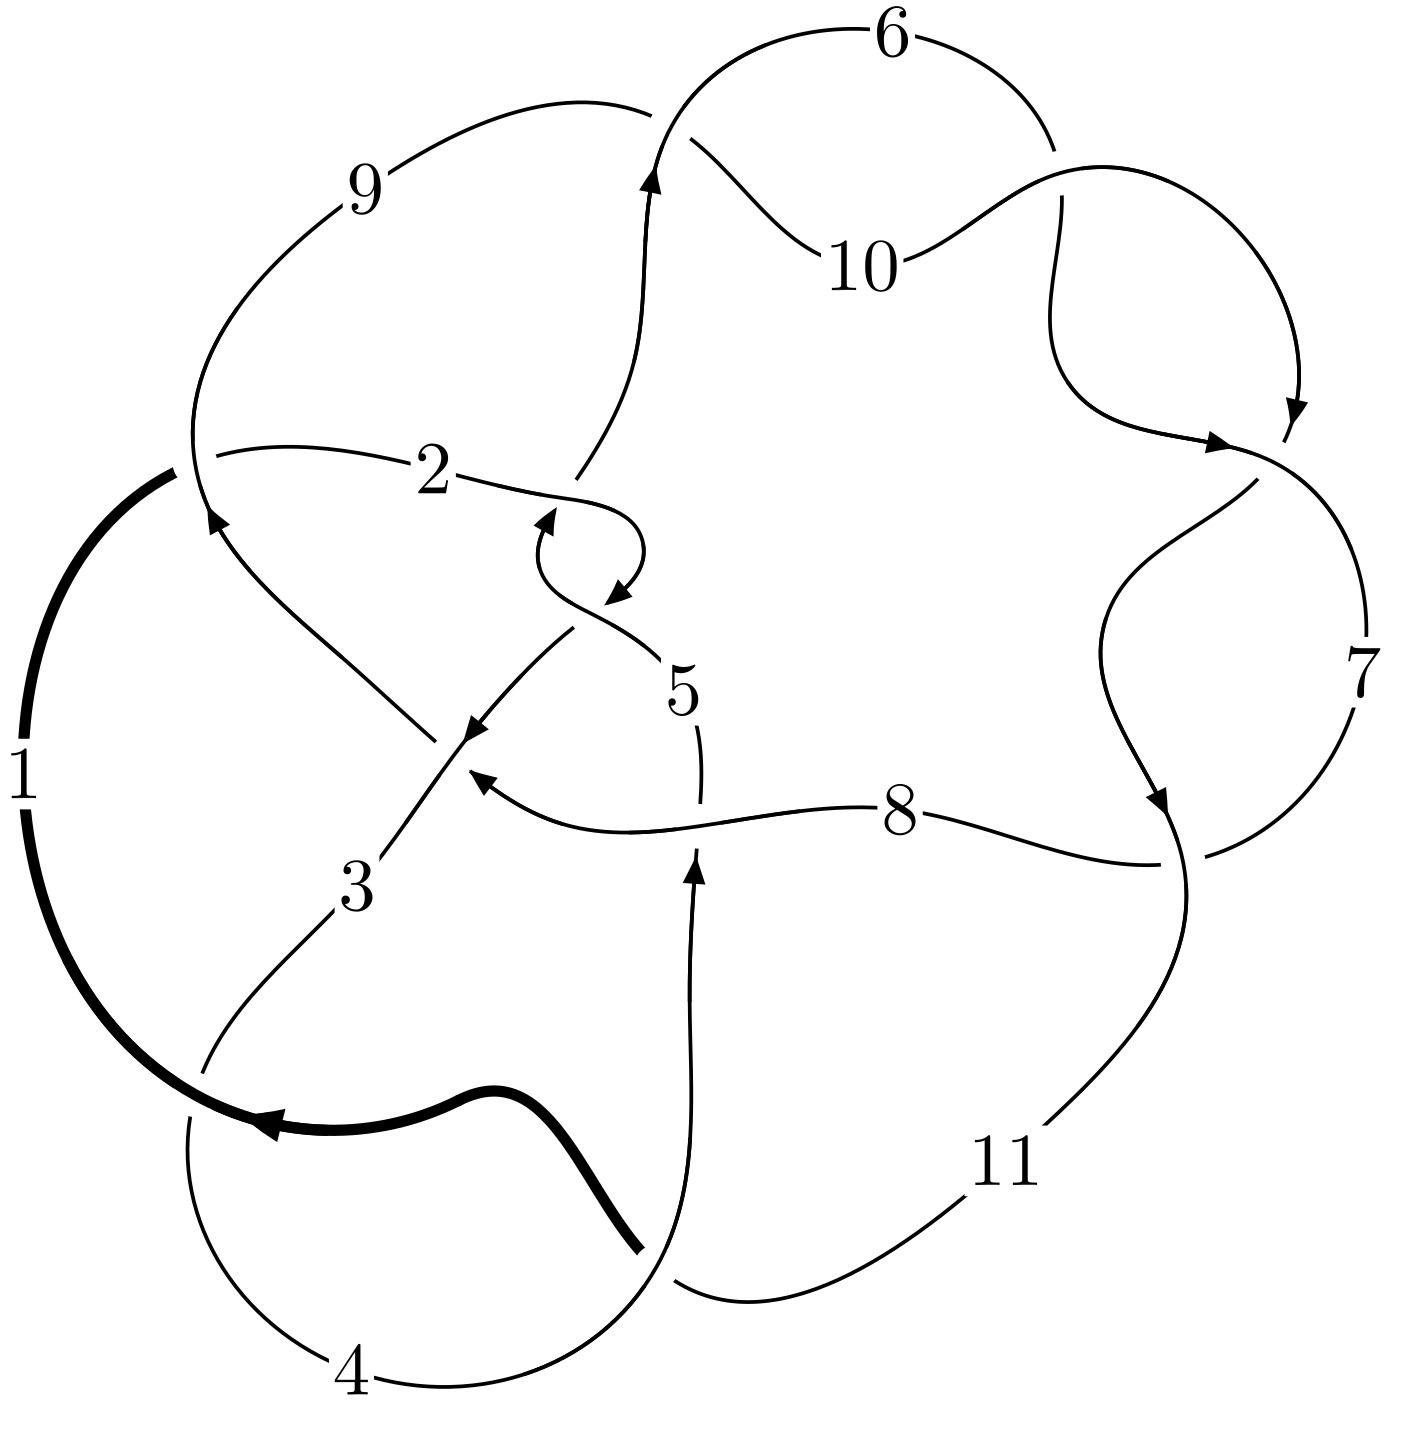
\includegraphics[width=112pt]{../../../GIT/diagram.site/Diagrams/png/542_11a_293.png}\\
\ \ \ A knot diagram\footnotemark}&
\allowdisplaybreaks
\textbf{Linearized knot diagam} \\
\cline{2-2}
 &
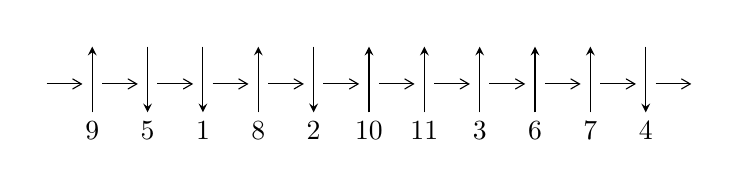
\begin{tikzpicture}[x=20pt, y=17pt]
	% nodes
	\node (C0) at (0, 0) {};
	\node (C1) at (1, 0) {};
	\node (C1U) at (1, +1) {};
	\node (C1D) at (1, -1) {9};

	\node (C2) at (2, 0) {};
	\node (C2U) at (2, +1) {};
	\node (C2D) at (2, -1) {5};

	\node (C3) at (3, 0) {};
	\node (C3U) at (3, +1) {};
	\node (C3D) at (3, -1) {1};

	\node (C4) at (4, 0) {};
	\node (C4U) at (4, +1) {};
	\node (C4D) at (4, -1) {8};

	\node (C5) at (5, 0) {};
	\node (C5U) at (5, +1) {};
	\node (C5D) at (5, -1) {2};

	\node (C6) at (6, 0) {};
	\node (C6U) at (6, +1) {};
	\node (C6D) at (6, -1) {10};

	\node (C7) at (7, 0) {};
	\node (C7U) at (7, +1) {};
	\node (C7D) at (7, -1) {11};

	\node (C8) at (8, 0) {};
	\node (C8U) at (8, +1) {};
	\node (C8D) at (8, -1) {3};

	\node (C9) at (9, 0) {};
	\node (C9U) at (9, +1) {};
	\node (C9D) at (9, -1) {6};

	\node (C10) at (10, 0) {};
	\node (C10U) at (10, +1) {};
	\node (C10D) at (10, -1) {7};

	\node (C11) at (11, 0) {};
	\node (C11U) at (11, +1) {};
	\node (C11D) at (11, -1) {4};
	\node (C12) at (12, 0) {};

	% arrows
	\draw[->,>={angle 60}]
	(C0) edge (C1) (C1) edge (C2) (C2) edge (C3) (C3) edge (C4) (C4) edge (C5) (C5) edge (C6) (C6) edge (C7) (C7) edge (C8) (C8) edge (C9) (C9) edge (C10) (C10) edge (C11) (C11) edge (C12) ;	\draw[->,>=stealth]
	(C1D) edge (C1U) (C2U) edge (C2D) (C3U) edge (C3D) (C4D) edge (C4U) (C5U) edge (C5D) (C6D) edge (C6U) (C7D) edge (C7U) (C8D) edge (C8U) (C9D) edge (C9U) (C10D) edge (C10U) (C11U) edge (C11D) ;
	\end{tikzpicture} \\
\hhline{~~} \\& 
\textbf{Solving Sequence} \\ \cline{2-2} 
 &
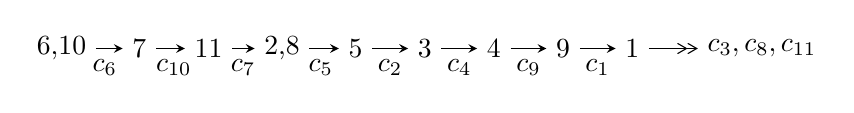
\begin{tikzpicture}[x=25pt, y=7pt]
	% node
	\node (A0) at (-1/8, 0) {6,10};
	\node (A1) at (1, 0) {7};
	\node (A2) at (2, 0) {11};
	\node (A3) at (49/16, 0) {2,8};
	\node (A4) at (33/8, 0) {5};
	\node (A5) at (41/8, 0) {3};
	\node (A6) at (49/8, 0) {4};
	\node (A7) at (57/8, 0) {9};
	\node (A8) at (65/8, 0) {1};
	\node (C1) at (1/2, -1) {$c_{6}$};
	\node (C2) at (3/2, -1) {$c_{10}$};
	\node (C3) at (5/2, -1) {$c_{7}$};
	\node (C4) at (29/8, -1) {$c_{5}$};
	\node (C5) at (37/8, -1) {$c_{2}$};
	\node (C6) at (45/8, -1) {$c_{4}$};
	\node (C7) at (53/8, -1) {$c_{9}$};
	\node (C8) at (61/8, -1) {$c_{1}$};
	\node (A9) at (10, 0) {$c_{3},c_{8},c_{11}$};

	% edge
	\draw[->,>=stealth]	
	(A0) edge (A1) (A1) edge (A2) (A2) edge (A3) (A3) edge (A4) (A4) edge (A5) (A5) edge (A6) (A6) edge (A7) (A7) edge (A8) ;
	\draw[->>,>={angle 60}]	
	(A8) edge (A9);
\end{tikzpicture} \\ 

\end{tabular} \\

\footnotetext{
The image of knot diagram is generated by the software ``\textbf{Draw programme}" developed by Andrew Bartholomew(\url{http://www.layer8.co.uk/maths/draw/index.htm\#Running-draw}), where we modified some parts for our purpose(\url{https://github.com/CATsTAILs/LinksPainter}).
}\phantom \\ \newline 
\centering \textbf{Ideals for irreducible components\footnotemark of $X_{\text{par}}$} 
 
\begin{align*}
I^u_{1}&=\langle 
913 u^{13}+2065 u^{12}+\cdots+8482 b+8631,\;-2839 u^{13}-4303 u^{12}+\cdots+8482 a-12824,\\
\phantom{I^u_{1}}&\phantom{= \langle  }u^{14}-8 u^{12}+u^{11}+22 u^{10}-6 u^9-21 u^8+8 u^7-3 u^6+10 u^5+15 u^4-16 u^3- u^2+3 u-1\rangle \\
I^u_{2}&=\langle 
6 u^{11} a+15 u^{11}+\cdots-8 a+49,\;-6 u^{11} a+24 u^{11}+\cdots-16 a+61,\\
\phantom{I^u_{2}}&\phantom{= \langle  }u^{12}+2 u^{11}-6 u^{10}-13 u^9+10 u^8+27 u^7- u^6-19 u^5-7 u^4+3 u^3+5 u^2+4 u+1\rangle \\
I^u_{3}&=\langle 
- u^3- u^2+b+2 u+3,\;3 u^3+2 u^2+4 a-7 u-7,\;u^4+2 u^3- u^2-5 u-4\rangle \\
I^u_{4}&=\langle 
b+a-1,\;a^2- a+2,\;u-1\rangle \\
I^u_{5}&=\langle 
b+1,\;2 a-1,\;u^2- u-1\rangle \\
I^u_{6}&=\langle 
2 b+a-1,\;a^2-2 a+5,\;u+1\rangle \\
\\
\end{align*}
\raggedright * 6 irreducible components of $\dim_{\mathbb{C}}=0$, with total 48 representations.\\
\footnotetext{All coefficients of polynomials are rational numbers. But the coefficients are sometimes approximated in decimal forms when there is not enough margin.}
\newpage
\renewcommand{\arraystretch}{1}
\centering \section*{I. $I^u_{1}= \langle 913 u^{13}+2065 u^{12}+\cdots+8482 b+8631,\;-2839 u^{13}-4303 u^{12}+\cdots+8482 a-12824,\;u^{14}-8 u^{12}+\cdots+3 u-1 \rangle$}
\flushleft \textbf{(i) Arc colorings}\\
\begin{tabular}{m{7pt} m{180pt} m{7pt} m{180pt} }
\flushright $a_{6}=$&$\begin{pmatrix}1\\0\end{pmatrix}$ \\
\flushright $a_{10}=$&$\begin{pmatrix}0\\u\end{pmatrix}$ \\
\flushright $a_{7}=$&$\begin{pmatrix}1\\- u^2\end{pmatrix}$ \\
\flushright $a_{11}=$&$\begin{pmatrix}u\\- u^3+u\end{pmatrix}$ \\
\flushright $a_{2}=$&$\begin{pmatrix}0.334709 u^{13}+0.507310 u^{12}+\cdots-4.54692 u+1.51191\\-0.107640 u^{13}-0.243457 u^{12}+\cdots+0.643480 u-1.01757\end{pmatrix}$ \\
\flushright $a_{8}=$&$\begin{pmatrix}- u^2+1\\u^4-2 u^2\end{pmatrix}$ \\
\flushright $a_{5}=$&$\begin{pmatrix}0.319264 u^{13}+0.439519 u^{12}+\cdots-2.93433 u+1.63535\\-0.298750 u^{13}-0.387644 u^{12}+\cdots+1.39165 u-0.986324\end{pmatrix}$ \\
\flushright $a_{3}=$&$\begin{pmatrix}0.910988 u^{13}+0.884108 u^{12}+\cdots-6.82056 u+2.65798\\-0.596793 u^{13}-0.428672 u^{12}+\cdots+1.81632 u-1.79510\end{pmatrix}$ \\
\flushright $a_{4}=$&$\begin{pmatrix}0.510257 u^{13}+0.525937 u^{12}+\cdots-4.02134 u+2.07451\\-0.216576 u^{13}-0.122377 u^{12}+\cdots+0.559774 u-0.860646\end{pmatrix}$ \\
\flushright $a_{9}=$&$\begin{pmatrix}- u\\u\end{pmatrix}$ \\
\flushright $a_{1}=$&$\begin{pmatrix}0.546805 u^{13}+0.434449 u^{12}+\cdots-3.98243 u+1.24805\\-0.319736 u^{13}-0.170597 u^{12}+\cdots+0.0789908 u-0.753714\end{pmatrix}$\\ \flushright $a_{1}=$&$\begin{pmatrix}0.546805 u^{13}+0.434449 u^{12}+\cdots-3.98243 u+1.24805\\-0.319736 u^{13}-0.170597 u^{12}+\cdots+0.0789908 u-0.753714\end{pmatrix}$\\&\end{tabular}
\flushleft \textbf{(ii) Obstruction class $= -1$}\\~\\
\flushleft \textbf{(iii) Cusp Shapes $= \frac{16306}{4241} u^{13}+\frac{88645}{16964} u^{12}+\cdots-\frac{152282}{4241} u+\frac{157881}{16964}$}\\~\\
\newpage\renewcommand{\arraystretch}{1}
\flushleft \textbf{(iv) u-Polynomials at the component}\newline \\
\begin{tabular}{m{50pt}|m{274pt}}
Crossings & \hspace{64pt}u-Polynomials at each crossing \\
\hline $$\begin{aligned}c_{1},c_{4}\end{aligned}$$&$\begin{aligned}
&4(4 u^{14}-22 u^{13}+\cdots-12 u+2)
\end{aligned}$\\
\hline $$\begin{aligned}c_{2},c_{3},c_{5}\\c_{11}\end{aligned}$$&$\begin{aligned}
&u^{14}+u^{13}+\cdots+4 u-1
\end{aligned}$\\
\hline $$\begin{aligned}c_{6},c_{7},c_{9}\\c_{10}\end{aligned}$$&$\begin{aligned}
&u^{14}-8 u^{12}+\cdots-3 u-1
\end{aligned}$\\
\hline $$\begin{aligned}c_{8}\end{aligned}$$&$\begin{aligned}
&u^{14}+5 u^{13}+\cdots-44 u+16
\end{aligned}$\\
\hline
\end{tabular}\\~\\
\newpage\renewcommand{\arraystretch}{1}
\flushleft \textbf{(v) Riley Polynomials at the component}\newline \\
\begin{tabular}{m{50pt}|m{274pt}}
Crossings & \hspace{64pt}Riley Polynomials at each crossing \\
\hline $$\begin{aligned}c_{1},c_{4}\end{aligned}$$&$\begin{aligned}
&16(16 y^{14}-172 y^{13}+\cdots-148 y^2+4)
\end{aligned}$\\
\hline $$\begin{aligned}c_{2},c_{3},c_{5}\\c_{11}\end{aligned}$$&$\begin{aligned}
&y^{14}+13 y^{13}+\cdots-54 y+1
\end{aligned}$\\
\hline $$\begin{aligned}c_{6},c_{7},c_{9}\\c_{10}\end{aligned}$$&$\begin{aligned}
&y^{14}-16 y^{13}+\cdots-7 y+1
\end{aligned}$\\
\hline $$\begin{aligned}c_{8}\end{aligned}$$&$\begin{aligned}
&y^{14}- y^{13}+\cdots-1584 y+256
\end{aligned}$\\
\hline
\end{tabular}\\~\\
\newpage\flushleft \textbf{(vi) Complex Volumes and Cusp Shapes}
$$\begin{array}{c|c|c}  
\text{Solutions to }I^u_{1}& \I (\text{vol} + \sqrt{-1}CS) & \text{Cusp shape}\\
 \hline 
\begin{aligned}
u &= -0.120466 + 0.916470 I \\
a &= \phantom{-}0.368601 - 0.148138 I \\
b &= \phantom{-}0.258574 + 1.300320 I\end{aligned}
 & \phantom{-}5.81499 - 5.60499 I & \phantom{-}9.56216 + 5.32481 I \\ \hline\begin{aligned}
u &= -0.120466 - 0.916470 I \\
a &= \phantom{-}0.368601 + 0.148138 I \\
b &= \phantom{-}0.258574 - 1.300320 I\end{aligned}
 & \phantom{-}5.81499 + 5.60499 I & \phantom{-}9.56216 - 5.32481 I \\ \hline\begin{aligned}
u &= \phantom{-}1.016760 + 0.568716 I \\
a &= \phantom{-}0.96711 + 1.31824 I \\
b &= \phantom{-}0.41976 - 1.38103 I\end{aligned}
 & \phantom{-}9.30919 + 10.50750 I & \phantom{-}10.66498 - 7.31370 I \\ \hline\begin{aligned}
u &= \phantom{-}1.016760 - 0.568716 I \\
a &= \phantom{-}0.96711 - 1.31824 I \\
b &= \phantom{-}0.41976 + 1.38103 I\end{aligned}
 & \phantom{-}9.30919 - 10.50750 I & \phantom{-}10.66498 + 7.31370 I \\ \hline\begin{aligned}
u &= \phantom{-}0.737410\phantom{ +0.000000I} \\
a &= \phantom{-}0.467940\phantom{ +0.000000I} \\
b &= -1.22694\phantom{ +0.000000I}\end{aligned}
 & -0.355949\phantom{ +0.000000I} & \phantom{-}22.0910\phantom{ +0.000000I} \\ \hline\begin{aligned}
u &= -1.309190 + 0.052676 I \\
a &= \phantom{-}0.259567 - 1.228370 I \\
b &= -0.364310 + 0.747897 I\end{aligned}
 & \phantom{-}3.65387 + 1.40001 I & \phantom{-}5.70050 - 4.92983 I \\ \hline\begin{aligned}
u &= -1.309190 - 0.052676 I \\
a &= \phantom{-}0.259567 + 1.228370 I \\
b &= -0.364310 - 0.747897 I\end{aligned}
 & \phantom{-}3.65387 - 1.40001 I & \phantom{-}5.70050 + 4.92983 I \\ \hline\begin{aligned}
u &= -0.526573\phantom{ +0.000000I} \\
a &= \phantom{-}0.667838\phantom{ +0.000000I} \\
b &= \phantom{-}0.133734\phantom{ +0.000000I}\end{aligned}
 & \phantom{-}0.784313\phantom{ +0.000000I} & \phantom{-}13.0950\phantom{ +0.000000I} \\ \hline\begin{aligned}
u &= \phantom{-}0.268307 + 0.257341 I \\
a &= -0.233314 - 1.367320 I \\
b &= -0.644907 + 0.288035 I\end{aligned}
 & -1.20190 + 0.85736 I & -4.43900 - 4.77044 I \\ \hline\begin{aligned}
u &= \phantom{-}0.268307 - 0.257341 I \\
a &= -0.233314 + 1.367320 I \\
b &= -0.644907 - 0.288035 I\end{aligned}
 & -1.20190 - 0.85736 I & -4.43900 + 4.77044 I\\
 \hline 
 \end{array}$$\newpage$$\begin{array}{c|c|c}  
\text{Solutions to }I^u_{1}& \I (\text{vol} + \sqrt{-1}CS) & \text{Cusp shape}\\
 \hline 
\begin{aligned}
u &= -1.72014 + 0.16032 I \\
a &= \phantom{-}0.52732 - 1.89025 I \\
b &= \phantom{-}0.52839 + 1.47236 I\end{aligned}
 & \phantom{-}18.7924 - 13.4596 I & \phantom{-}11.49654 + 6.20510 I \\ \hline\begin{aligned}
u &= -1.72014 - 0.16032 I \\
a &= \phantom{-}0.52732 + 1.89025 I \\
b &= \phantom{-}0.52839 - 1.47236 I\end{aligned}
 & \phantom{-}18.7924 + 13.4596 I & \phantom{-}11.49654 - 6.20510 I \\ \hline\begin{aligned}
u &= \phantom{-}1.75930 + 0.20189 I \\
a &= -0.45717 - 1.59729 I \\
b &= -0.150905 + 1.395380 I\end{aligned}
 & \phantom{-}17.7001 + 3.9528 I & \phantom{-}13.79713 - 2.45311 I \\ \hline\begin{aligned}
u &= \phantom{-}1.75930 - 0.20189 I \\
a &= -0.45717 + 1.59729 I \\
b &= -0.150905 - 1.395380 I\end{aligned}
 & \phantom{-}17.7001 - 3.9528 I & \phantom{-}13.79713 + 2.45311 I\\
 \hline 
 \end{array}$$\newpage\newpage\renewcommand{\arraystretch}{1}
\centering \section*{II. $I^u_{2}= \langle 6 u^{11} a+15 u^{11}+\cdots-8 a+49,\;-6 u^{11} a+24 u^{11}+\cdots-16 a+61,\;u^{12}+2 u^{11}+\cdots+4 u+1 \rangle$}
\flushleft \textbf{(i) Arc colorings}\\
\begin{tabular}{m{7pt} m{180pt} m{7pt} m{180pt} }
\flushright $a_{6}=$&$\begin{pmatrix}1\\0\end{pmatrix}$ \\
\flushright $a_{10}=$&$\begin{pmatrix}0\\u\end{pmatrix}$ \\
\flushright $a_{7}=$&$\begin{pmatrix}1\\- u^2\end{pmatrix}$ \\
\flushright $a_{11}=$&$\begin{pmatrix}u\\- u^3+u\end{pmatrix}$ \\
\flushright $a_{2}=$&$\begin{pmatrix}a\\-0.260870 a u^{11}-0.652174 u^{11}+\cdots+0.347826 a-2.13043\end{pmatrix}$ \\
\flushright $a_{8}=$&$\begin{pmatrix}- u^2+1\\u^4-2 u^2\end{pmatrix}$ \\
\flushright $a_{5}=$&$\begin{pmatrix}-0.652174 a u^{11}+7.86957 u^{11}+\cdots-2.13043 a+19.1739\\-0.304348 a u^{11}-0.260870 u^{11}+\cdots-0.260870 a+1.34783\end{pmatrix}$ \\
\flushright $a_{3}=$&$\begin{pmatrix}-2 u^{11}- u^{10}+\cdots-4 u-2\\2 u^{11}-13 u^9+27 u^7+u^6-19 u^5-4 u^4+3 u^3+3 u^2+4 u+1\end{pmatrix}$ \\
\flushright $a_{4}=$&$\begin{pmatrix}-0.347826 a u^{11}+4.13043 u^{11}+\cdots-1.86957 a+12.8261\\-0.304348 a u^{11}+3.73913 u^{11}+\cdots-0.260870 a+5.34783\end{pmatrix}$ \\
\flushright $a_{9}=$&$\begin{pmatrix}- u\\u\end{pmatrix}$ \\
\flushright $a_{1}=$&$\begin{pmatrix}0.521739 a u^{11}+0.304348 u^{11}+\cdots+1.30435 a+0.260870\\-0.782609 a u^{11}-0.956522 u^{11}+\cdots+0.0434783 a-2.39130\end{pmatrix}$\\ \flushright $a_{1}=$&$\begin{pmatrix}0.521739 a u^{11}+0.304348 u^{11}+\cdots+1.30435 a+0.260870\\-0.782609 a u^{11}-0.956522 u^{11}+\cdots+0.0434783 a-2.39130\end{pmatrix}$\\&\end{tabular}
\flushleft \textbf{(ii) Obstruction class $= -1$}\\~\\
\flushleft \textbf{(iii) Cusp Shapes $= 4 u^{10}-28 u^8+64 u^6+4 u^5-52 u^4-16 u^3+12 u^2+12 u+14$}\\~\\
\newpage\renewcommand{\arraystretch}{1}
\flushleft \textbf{(iv) u-Polynomials at the component}\newline \\
\begin{tabular}{m{50pt}|m{274pt}}
Crossings & \hspace{64pt}u-Polynomials at each crossing \\
\hline $$\begin{aligned}c_{1},c_{4}\end{aligned}$$&$\begin{aligned}
&u^{24}-7 u^{23}+\cdots-5492 u+2488
\end{aligned}$\\
\hline $$\begin{aligned}c_{2},c_{3},c_{5}\\c_{11}\end{aligned}$$&$\begin{aligned}
&u^{24}-4 u^{23}+\cdots-4 u+1
\end{aligned}$\\
\hline $$\begin{aligned}c_{6},c_{7},c_{9}\\c_{10}\end{aligned}$$&$\begin{aligned}
&(u^{12}-2 u^{11}+\cdots-4 u+1)^{2}
\end{aligned}$\\
\hline $$\begin{aligned}c_{8}\end{aligned}$$&$\begin{aligned}
&(u^{12}-2 u^{10}+u^9+4 u^8- u^7-3 u^6+3 u^5+3 u^4- u^3- u^2+2 u+1)^2
\end{aligned}$\\
\hline
\end{tabular}\\~\\
\newpage\renewcommand{\arraystretch}{1}
\flushleft \textbf{(v) Riley Polynomials at the component}\newline \\
\begin{tabular}{m{50pt}|m{274pt}}
Crossings & \hspace{64pt}Riley Polynomials at each crossing \\
\hline $$\begin{aligned}c_{1},c_{4}\end{aligned}$$&$\begin{aligned}
&y^{24}-15 y^{23}+\cdots-39497040 y+6190144
\end{aligned}$\\
\hline $$\begin{aligned}c_{2},c_{3},c_{5}\\c_{11}\end{aligned}$$&$\begin{aligned}
&y^{24}+16 y^{23}+\cdots+20 y+1
\end{aligned}$\\
\hline $$\begin{aligned}c_{6},c_{7},c_{9}\\c_{10}\end{aligned}$$&$\begin{aligned}
&(y^{12}-16 y^{11}+\cdots-6 y+1)^{2}
\end{aligned}$\\
\hline $$\begin{aligned}c_{8}\end{aligned}$$&$\begin{aligned}
&(y^{12}-4 y^{11}+\cdots-6 y+1)^{2}
\end{aligned}$\\
\hline
\end{tabular}\\~\\
\newpage\flushleft \textbf{(vi) Complex Volumes and Cusp Shapes}
$$\begin{array}{c|c|c}  
\text{Solutions to }I^u_{2}& \I (\text{vol} + \sqrt{-1}CS) & \text{Cusp shape}\\
 \hline 
\begin{aligned}
u &= \phantom{-}0.906692 + 0.344889 I \\
a &= \phantom{-}0.087956 + 0.330963 I \\
b &= \phantom{-}0.991263 - 0.128941 I\end{aligned}
 & \phantom{-}4.52195 + 5.52285 I & \phantom{-}8.56374 - 6.48307 I \\ \hline\begin{aligned}
u &= \phantom{-}0.906692 + 0.344889 I \\
a &= -0.87713 - 1.53641 I \\
b &= -0.42275 + 1.37969 I\end{aligned}
 & \phantom{-}4.52195 + 5.52285 I & \phantom{-}8.56374 - 6.48307 I \\ \hline\begin{aligned}
u &= \phantom{-}0.906692 - 0.344889 I \\
a &= \phantom{-}0.087956 - 0.330963 I \\
b &= \phantom{-}0.991263 + 0.128941 I\end{aligned}
 & \phantom{-}4.52195 - 5.52285 I & \phantom{-}8.56374 + 6.48307 I \\ \hline\begin{aligned}
u &= \phantom{-}0.906692 - 0.344889 I \\
a &= -0.87713 + 1.53641 I \\
b &= -0.42275 - 1.37969 I\end{aligned}
 & \phantom{-}4.52195 - 5.52285 I & \phantom{-}8.56374 + 6.48307 I \\ \hline\begin{aligned}
u &= -0.746978 + 0.302047 I \\
a &= -0.486446 - 1.164460 I \\
b &= -0.009071 - 0.303466 I\end{aligned}
 & \phantom{-}3.49764 - 0.49850 I & \phantom{-}6.63137 + 1.38008 I \\ \hline\begin{aligned}
u &= -0.746978 + 0.302047 I \\
a &= \phantom{-}1.74786 - 1.42100 I \\
b &= \phantom{-}0.002396 + 1.116620 I\end{aligned}
 & \phantom{-}3.49764 - 0.49850 I & \phantom{-}6.63137 + 1.38008 I \\ \hline\begin{aligned}
u &= -0.746978 - 0.302047 I \\
a &= -0.486446 + 1.164460 I \\
b &= -0.009071 + 0.303466 I\end{aligned}
 & \phantom{-}3.49764 + 0.49850 I & \phantom{-}6.63137 - 1.38008 I \\ \hline\begin{aligned}
u &= -0.746978 - 0.302047 I \\
a &= \phantom{-}1.74786 + 1.42100 I \\
b &= \phantom{-}0.002396 - 1.116620 I\end{aligned}
 & \phantom{-}3.49764 + 0.49850 I & \phantom{-}6.63137 - 1.38008 I \\ \hline\begin{aligned}
u &= -0.077590 + 0.553195 I \\
a &= \phantom{-}0.931659 + 0.876936 I \\
b &= \phantom{-}0.580478 + 0.088669 I\end{aligned}
 & \phantom{-}1.52068 - 2.46907 I & \phantom{-}2.47747 + 3.95252 I \\ \hline\begin{aligned}
u &= -0.077590 + 0.553195 I \\
a &= -0.188696 - 0.434891 I \\
b &= -0.255684 - 1.161480 I\end{aligned}
 & \phantom{-}1.52068 - 2.46907 I & \phantom{-}2.47747 + 3.95252 I\\
 \hline 
 \end{array}$$\newpage$$\begin{array}{c|c|c}  
\text{Solutions to }I^u_{2}& \I (\text{vol} + \sqrt{-1}CS) & \text{Cusp shape}\\
 \hline 
\begin{aligned}
u &= -0.077590 - 0.553195 I \\
a &= \phantom{-}0.931659 - 0.876936 I \\
b &= \phantom{-}0.580478 - 0.088669 I\end{aligned}
 & \phantom{-}1.52068 + 2.46907 I & \phantom{-}2.47747 - 3.95252 I \\ \hline\begin{aligned}
u &= -0.077590 - 0.553195 I \\
a &= -0.188696 + 0.434891 I \\
b &= -0.255684 + 1.161480 I\end{aligned}
 & \phantom{-}1.52068 + 2.46907 I & \phantom{-}2.47747 - 3.95252 I \\ \hline\begin{aligned}
u &= -0.389319\phantom{ +0.000000I} \\
a &= \phantom{-}4.87987 + 3.31193 I \\
b &= \phantom{-}0.110618 + 1.018190 I\end{aligned}
 & \phantom{-}3.95056\phantom{ +0.000000I} & \phantom{-}11.0690\phantom{ +0.000000I} \\ \hline\begin{aligned}
u &= -0.389319\phantom{ +0.000000I} \\
a &= \phantom{-}4.87987 - 3.31193 I \\
b &= \phantom{-}0.110618 - 1.018190 I\end{aligned}
 & \phantom{-}3.95056\phantom{ +0.000000I} & \phantom{-}11.0690\phantom{ +0.000000I} \\ \hline\begin{aligned}
u &= \phantom{-}1.65757 + 0.05967 I \\
a &= -0.425611 + 0.080237 I \\
b &= -0.498557 + 0.415422 I\end{aligned}
 & \phantom{-}11.96400 + 1.70959 I & \phantom{-}7.87181 - 0.16720 I \\ \hline\begin{aligned}
u &= \phantom{-}1.65757 + 0.05967 I \\
a &= \phantom{-}0.70856 + 2.24798 I \\
b &= \phantom{-}0.099763 - 1.246630 I\end{aligned}
 & \phantom{-}11.96400 + 1.70959 I & \phantom{-}7.87181 - 0.16720 I \\ \hline\begin{aligned}
u &= \phantom{-}1.65757 - 0.05967 I \\
a &= -0.425611 - 0.080237 I \\
b &= -0.498557 - 0.415422 I\end{aligned}
 & \phantom{-}11.96400 - 1.70959 I & \phantom{-}7.87181 + 0.16720 I \\ \hline\begin{aligned}
u &= \phantom{-}1.65757 - 0.05967 I \\
a &= \phantom{-}0.70856 - 2.24798 I \\
b &= \phantom{-}0.099763 + 1.246630 I\end{aligned}
 & \phantom{-}11.96400 - 1.70959 I & \phantom{-}7.87181 + 0.16720 I \\ \hline\begin{aligned}
u &= -1.68947 + 0.08890 I \\
a &= -0.548076 - 0.328965 I \\
b &= \phantom{-}1.265990 + 0.145887 I\end{aligned}
 & \phantom{-}13.6389 - 7.2036 I & \phantom{-}10.08749 + 4.71657 I \\ \hline\begin{aligned}
u &= -1.68947 + 0.08890 I \\
a &= -0.27673 + 2.03323 I \\
b &= -0.53950 - 1.55444 I\end{aligned}
 & \phantom{-}13.6389 - 7.2036 I & \phantom{-}10.08749 + 4.71657 I\\
 \hline 
 \end{array}$$\newpage$$\begin{array}{c|c|c}  
\text{Solutions to }I^u_{2}& \I (\text{vol} + \sqrt{-1}CS) & \text{Cusp shape}\\
 \hline 
\begin{aligned}
u &= -1.68947 - 0.08890 I \\
a &= -0.548076 + 0.328965 I \\
b &= \phantom{-}1.265990 - 0.145887 I\end{aligned}
 & \phantom{-}13.6389 + 7.2036 I & \phantom{-}10.08749 - 4.71657 I \\ \hline\begin{aligned}
u &= -1.68947 - 0.08890 I \\
a &= -0.27673 - 2.03323 I \\
b &= -0.53950 + 1.55444 I\end{aligned}
 & \phantom{-}13.6389 + 7.2036 I & \phantom{-}10.08749 - 4.71657 I \\ \hline\begin{aligned}
u &= -1.71112\phantom{ +0.000000I} \\
a &= -0.05322 + 1.80943 I \\
b &= \phantom{-}0.67504 - 1.53852 I\end{aligned}
 & \phantom{-}17.8795\phantom{ +0.000000I} & \phantom{-}13.6670\phantom{ +0.000000I} \\ \hline\begin{aligned}
u &= -1.71112\phantom{ +0.000000I} \\
a &= -0.05322 - 1.80943 I \\
b &= \phantom{-}0.67504 + 1.53852 I\end{aligned}
 & \phantom{-}17.8795\phantom{ +0.000000I} & \phantom{-}13.6670\phantom{ +0.000000I}\\
 \hline 
 \end{array}$$\newpage\newpage\renewcommand{\arraystretch}{1}
\centering \section*{III. $I^u_{3}= \langle - u^3- u^2+b+2 u+3,\;3 u^3+2 u^2+4 a-7 u-7,\;u^4+2 u^3- u^2-5 u-4 \rangle$}
\flushleft \textbf{(i) Arc colorings}\\
\begin{tabular}{m{7pt} m{180pt} m{7pt} m{180pt} }
\flushright $a_{6}=$&$\begin{pmatrix}1\\0\end{pmatrix}$ \\
\flushright $a_{10}=$&$\begin{pmatrix}0\\u\end{pmatrix}$ \\
\flushright $a_{7}=$&$\begin{pmatrix}1\\- u^2\end{pmatrix}$ \\
\flushright $a_{11}=$&$\begin{pmatrix}u\\- u^3+u\end{pmatrix}$ \\
\flushright $a_{2}=$&$\begin{pmatrix}-\frac{3}{4} u^3-\frac{1}{2} u^2+\frac{7}{4} u+\frac{7}{4}\\u^3+u^2-2 u-3\end{pmatrix}$ \\
\flushright $a_{8}=$&$\begin{pmatrix}- u^2+1\\-2 u^3- u^2+5 u+4\end{pmatrix}$ \\
\flushright $a_{5}=$&$\begin{pmatrix}-\frac{1}{4} u^3+\frac{1}{2} u^2+\frac{1}{4} u+\frac{1}{4}\\u^3-2 u-1\end{pmatrix}$ \\
\flushright $a_{3}=$&$\begin{pmatrix}-\frac{3}{2} u^3- u^2+\frac{5}{2} u+\frac{9}{2}\\u^3- u-2\end{pmatrix}$ \\
\flushright $a_{4}=$&$\begin{pmatrix}-\frac{1}{4} u^3-\frac{1}{2} u^2+\frac{1}{4} u+\frac{5}{4}\\- u^3- u^2+3 u+3\end{pmatrix}$ \\
\flushright $a_{9}=$&$\begin{pmatrix}- u\\u\end{pmatrix}$ \\
\flushright $a_{1}=$&$\begin{pmatrix}-\frac{3}{4} u^3-\frac{1}{2} u^2+\frac{3}{4} u+\frac{7}{4}\\u^3+u^2- u-3\end{pmatrix}$\\ \flushright $a_{1}=$&$\begin{pmatrix}-\frac{3}{4} u^3-\frac{1}{2} u^2+\frac{3}{4} u+\frac{7}{4}\\u^3+u^2- u-3\end{pmatrix}$\\&\end{tabular}
\flushleft \textbf{(ii) Obstruction class $= -1$}\\~\\
\flushleft \textbf{(iii) Cusp Shapes $= 14$}\\~\\
\newpage\renewcommand{\arraystretch}{1}
\flushleft \textbf{(iv) u-Polynomials at the component}\newline \\
\begin{tabular}{m{50pt}|m{274pt}}
Crossings & \hspace{64pt}u-Polynomials at each crossing \\
\hline $$\begin{aligned}c_{1},c_{4}\end{aligned}$$&$\begin{aligned}
&(u+1)^4
\end{aligned}$\\
\hline $$\begin{aligned}c_{2},c_{3},c_{5}\\c_{11}\end{aligned}$$&$\begin{aligned}
&u^4+u^3+u^2+2 u-1
\end{aligned}$\\
\hline $$\begin{aligned}c_{6},c_{7},c_{9}\\c_{10}\end{aligned}$$&$\begin{aligned}
&u^4-2 u^3- u^2+5 u-4
\end{aligned}$\\
\hline $$\begin{aligned}c_{8}\end{aligned}$$&$\begin{aligned}
&u^4-2 u^3+u^2+5 u+2
\end{aligned}$\\
\hline
\end{tabular}\\~\\
\newpage\renewcommand{\arraystretch}{1}
\flushleft \textbf{(v) Riley Polynomials at the component}\newline \\
\begin{tabular}{m{50pt}|m{274pt}}
Crossings & \hspace{64pt}Riley Polynomials at each crossing \\
\hline $$\begin{aligned}c_{1},c_{4}\end{aligned}$$&$\begin{aligned}
&(y-1)^4
\end{aligned}$\\
\hline $$\begin{aligned}c_{2},c_{3},c_{5}\\c_{11}\end{aligned}$$&$\begin{aligned}
&y^4+y^3-5 y^2-6 y+1
\end{aligned}$\\
\hline $$\begin{aligned}c_{6},c_{7},c_{9}\\c_{10}\end{aligned}$$&$\begin{aligned}
&y^4-6 y^3+13 y^2-17 y+16
\end{aligned}$\\
\hline $$\begin{aligned}c_{8}\end{aligned}$$&$\begin{aligned}
&y^4-2 y^3+25 y^2-21 y+4
\end{aligned}$\\
\hline
\end{tabular}\\~\\
\newpage\flushleft \textbf{(vi) Complex Volumes and Cusp Shapes}
$$\begin{array}{c|c|c}  
\text{Solutions to }I^u_{3}& \I (\text{vol} + \sqrt{-1}CS) & \text{Cusp shape}\\
 \hline 
\begin{aligned}
u &= -0.964457 + 0.761911 I \\
a &= -0.699517 + 0.805292 I \\
b &= \phantom{-}0.061094 - 1.309640 I\end{aligned}
 & \phantom{-}8.22467\phantom{ +0.000000I} & \phantom{-}14.0000\phantom{ +0.000000I} \\ \hline\begin{aligned}
u &= -0.964457 - 0.761911 I \\
a &= -0.699517 - 0.805292 I \\
b &= \phantom{-}0.061094 + 1.309640 I\end{aligned}
 & \phantom{-}8.22467\phantom{ +0.000000I} & \phantom{-}14.0000\phantom{ +0.000000I} \\ \hline\begin{aligned}
u &= \phantom{-}1.59205\phantom{ +0.000000I} \\
a &= \phantom{-}0.242325\phantom{ +0.000000I} \\
b &= \phantom{-}0.385795\phantom{ +0.000000I}\end{aligned}
 & \phantom{-}8.22467\phantom{ +0.000000I} & \phantom{-}14.0000\phantom{ +0.000000I} \\ \hline\begin{aligned}
u &= -1.66314\phantom{ +0.000000I} \\
a &= \phantom{-}0.906709\phantom{ +0.000000I} \\
b &= -1.50798\phantom{ +0.000000I}\end{aligned}
 & \phantom{-}8.22467\phantom{ +0.000000I} & \phantom{-}14.0000\phantom{ +0.000000I}\\
 \hline 
 \end{array}$$\newpage\newpage\renewcommand{\arraystretch}{1}
\centering \section*{IV. $I^u_{4}= \langle b+a-1,\;a^2- a+2,\;u-1 \rangle$}
\flushleft \textbf{(i) Arc colorings}\\
\begin{tabular}{m{7pt} m{180pt} m{7pt} m{180pt} }
\flushright $a_{6}=$&$\begin{pmatrix}1\\0\end{pmatrix}$ \\
\flushright $a_{10}=$&$\begin{pmatrix}0\\1\end{pmatrix}$ \\
\flushright $a_{7}=$&$\begin{pmatrix}1\\-1\end{pmatrix}$ \\
\flushright $a_{11}=$&$\begin{pmatrix}1\\0\end{pmatrix}$ \\
\flushright $a_{2}=$&$\begin{pmatrix}a\\- a+1\end{pmatrix}$ \\
\flushright $a_{8}=$&$\begin{pmatrix}0\\-1\end{pmatrix}$ \\
\flushright $a_{5}=$&$\begin{pmatrix}-1\\a+1\end{pmatrix}$ \\
\flushright $a_{3}=$&$\begin{pmatrix}1\\-2\end{pmatrix}$ \\
\flushright $a_{4}=$&$\begin{pmatrix}-1\\a\end{pmatrix}$ \\
\flushright $a_{9}=$&$\begin{pmatrix}-1\\1\end{pmatrix}$ \\
\flushright $a_{1}=$&$\begin{pmatrix}a-1\\- a+2\end{pmatrix}$\\ \flushright $a_{1}=$&$\begin{pmatrix}a-1\\- a+2\end{pmatrix}$\\&\end{tabular}
\flushleft \textbf{(ii) Obstruction class $= -1$}\\~\\
\flushleft \textbf{(iii) Cusp Shapes $= 14$}\\~\\
\newpage\renewcommand{\arraystretch}{1}
\flushleft \textbf{(iv) u-Polynomials at the component}\newline \\
\begin{tabular}{m{50pt}|m{274pt}}
Crossings & \hspace{64pt}u-Polynomials at each crossing \\
\hline $$\begin{aligned}c_{1},c_{4},c_{6}\\c_{7},c_{9},c_{10}\end{aligned}$$&$\begin{aligned}
&(u+1)^2
\end{aligned}$\\
\hline $$\begin{aligned}c_{2},c_{3},c_{5}\\c_{11}\end{aligned}$$&$\begin{aligned}
&u^2- u+2
\end{aligned}$\\
\hline $$\begin{aligned}c_{8}\end{aligned}$$&$\begin{aligned}
&(u-1)^2
\end{aligned}$\\
\hline
\end{tabular}\\~\\
\newpage\renewcommand{\arraystretch}{1}
\flushleft \textbf{(v) Riley Polynomials at the component}\newline \\
\begin{tabular}{m{50pt}|m{274pt}}
Crossings & \hspace{64pt}Riley Polynomials at each crossing \\
\hline $$\begin{aligned}c_{1},c_{4},c_{6}\\c_{7},c_{8},c_{9}\\c_{10}\end{aligned}$$&$\begin{aligned}
&(y-1)^2
\end{aligned}$\\
\hline $$\begin{aligned}c_{2},c_{3},c_{5}\\c_{11}\end{aligned}$$&$\begin{aligned}
&y^2+3 y+4
\end{aligned}$\\
\hline
\end{tabular}\\~\\
\newpage\flushleft \textbf{(vi) Complex Volumes and Cusp Shapes}
$$\begin{array}{c|c|c}  
\text{Solutions to }I^u_{4}& \I (\text{vol} + \sqrt{-1}CS) & \text{Cusp shape}\\
 \hline 
\begin{aligned}
u &= \phantom{-}1.00000\phantom{ +0.000000I} \\
a &= \phantom{-}0.50000 + 1.32288 I \\
b &= \phantom{-}0.50000 - 1.32288 I\end{aligned}
 & \phantom{-}8.22467\phantom{ +0.000000I} & \phantom{-}14.0000\phantom{ +0.000000I} \\ \hline\begin{aligned}
u &= \phantom{-}1.00000\phantom{ +0.000000I} \\
a &= \phantom{-}0.50000 - 1.32288 I \\
b &= \phantom{-}0.50000 + 1.32288 I\end{aligned}
 & \phantom{-}8.22467\phantom{ +0.000000I} & \phantom{-}14.0000\phantom{ +0.000000I}\\
 \hline 
 \end{array}$$\newpage\newpage\renewcommand{\arraystretch}{1}
\centering \section*{V. $I^u_{5}= \langle b+1,\;2 a-1,\;u^2- u-1 \rangle$}
\flushleft \textbf{(i) Arc colorings}\\
\begin{tabular}{m{7pt} m{180pt} m{7pt} m{180pt} }
\flushright $a_{6}=$&$\begin{pmatrix}1\\0\end{pmatrix}$ \\
\flushright $a_{10}=$&$\begin{pmatrix}0\\u\end{pmatrix}$ \\
\flushright $a_{7}=$&$\begin{pmatrix}1\\- u-1\end{pmatrix}$ \\
\flushright $a_{11}=$&$\begin{pmatrix}u\\- u-1\end{pmatrix}$ \\
\flushright $a_{2}=$&$\begin{pmatrix}0.5\\-1\end{pmatrix}$ \\
\flushright $a_{8}=$&$\begin{pmatrix}- u\\u\end{pmatrix}$ \\
\flushright $a_{5}=$&$\begin{pmatrix}1.5\\-1\end{pmatrix}$ \\
\flushright $a_{3}=$&$\begin{pmatrix}2\\-2\end{pmatrix}$ \\
\flushright $a_{4}=$&$\begin{pmatrix}-\frac{1}{2} u+1\\\frac{1}{2} u-\frac{1}{2}\end{pmatrix}$ \\
\flushright $a_{9}=$&$\begin{pmatrix}- u\\u\end{pmatrix}$ \\
\flushright $a_{1}=$&$\begin{pmatrix}\frac{1}{2} u+1\\-\frac{1}{2} u-\frac{3}{2}\end{pmatrix}$\\ \flushright $a_{1}=$&$\begin{pmatrix}\frac{1}{2} u+1\\-\frac{1}{2} u-\frac{3}{2}\end{pmatrix}$\\&\end{tabular}
\flushleft \textbf{(ii) Obstruction class $= 1$}\\~\\
\flushleft \textbf{(iii) Cusp Shapes $= \frac{15}{4} u-\frac{9}{4}$}\\~\\
\newpage\renewcommand{\arraystretch}{1}
\flushleft \textbf{(iv) u-Polynomials at the component}\newline \\
\begin{tabular}{m{50pt}|m{274pt}}
Crossings & \hspace{64pt}u-Polynomials at each crossing \\
\hline $$\begin{aligned}c_{1}\end{aligned}$$&$\begin{aligned}
&4(4 u^2+2 u-1)
\end{aligned}$\\
\hline $$\begin{aligned}c_{2},c_{11}\end{aligned}$$&$\begin{aligned}
&(u-1)^2
\end{aligned}$\\
\hline $$\begin{aligned}c_{3},c_{5}\end{aligned}$$&$\begin{aligned}
&(u+1)^2
\end{aligned}$\\
\hline $$\begin{aligned}c_{4}\end{aligned}$$&$\begin{aligned}
&4(4 u^2-2 u-1)
\end{aligned}$\\
\hline $$\begin{aligned}c_{6},c_{7}\end{aligned}$$&$\begin{aligned}
&u^2- u-1
\end{aligned}$\\
\hline $$\begin{aligned}c_{8}\end{aligned}$$&$\begin{aligned}
&u^2
\end{aligned}$\\
\hline $$\begin{aligned}c_{9},c_{10}\end{aligned}$$&$\begin{aligned}
&u^2+u-1
\end{aligned}$\\
\hline
\end{tabular}\\~\\
\newpage\renewcommand{\arraystretch}{1}
\flushleft \textbf{(v) Riley Polynomials at the component}\newline \\
\begin{tabular}{m{50pt}|m{274pt}}
Crossings & \hspace{64pt}Riley Polynomials at each crossing \\
\hline $$\begin{aligned}c_{1},c_{4}\end{aligned}$$&$\begin{aligned}
&16(16 y^2-12 y+1)
\end{aligned}$\\
\hline $$\begin{aligned}c_{2},c_{3},c_{5}\\c_{11}\end{aligned}$$&$\begin{aligned}
&(y-1)^2
\end{aligned}$\\
\hline $$\begin{aligned}c_{6},c_{7},c_{9}\\c_{10}\end{aligned}$$&$\begin{aligned}
&y^2-3 y+1
\end{aligned}$\\
\hline $$\begin{aligned}c_{8}\end{aligned}$$&$\begin{aligned}
&y^2
\end{aligned}$\\
\hline
\end{tabular}\\~\\
\newpage\flushleft \textbf{(vi) Complex Volumes and Cusp Shapes}
$$\begin{array}{c|c|c}  
\text{Solutions to }I^u_{5}& \I (\text{vol} + \sqrt{-1}CS) & \text{Cusp shape}\\
 \hline 
\begin{aligned}
u &= -0.618034\phantom{ +0.000000I} \\
a &= \phantom{-}0.500000\phantom{ +0.000000I} \\
b &= -1.00000\phantom{ +0.000000I}\end{aligned}
 & -0.657974\phantom{ +0.000000I} & -4.56760\phantom{ +0.000000I} \\ \hline\begin{aligned}
u &= \phantom{-}1.61803\phantom{ +0.000000I} \\
a &= \phantom{-}0.500000\phantom{ +0.000000I} \\
b &= -1.00000\phantom{ +0.000000I}\end{aligned}
 & \phantom{-}7.23771\phantom{ +0.000000I} & \phantom{-}3.81760\phantom{ +0.000000I}\\
 \hline 
 \end{array}$$\newpage\newpage\renewcommand{\arraystretch}{1}
\centering \section*{VI. $I^u_{6}= \langle 2 b+a-1,\;a^2-2 a+5,\;u+1 \rangle$}
\flushleft \textbf{(i) Arc colorings}\\
\begin{tabular}{m{7pt} m{180pt} m{7pt} m{180pt} }
\flushright $a_{6}=$&$\begin{pmatrix}1\\0\end{pmatrix}$ \\
\flushright $a_{10}=$&$\begin{pmatrix}0\\-1\end{pmatrix}$ \\
\flushright $a_{7}=$&$\begin{pmatrix}1\\-1\end{pmatrix}$ \\
\flushright $a_{11}=$&$\begin{pmatrix}-1\\0\end{pmatrix}$ \\
\flushright $a_{2}=$&$\begin{pmatrix}a\\-\frac{1}{2} a+\frac{1}{2}\end{pmatrix}$ \\
\flushright $a_{8}=$&$\begin{pmatrix}0\\-1\end{pmatrix}$ \\
\flushright $a_{5}=$&$\begin{pmatrix}\frac{1}{2} a-\frac{3}{2}\\1\end{pmatrix}$ \\
\flushright $a_{3}=$&$\begin{pmatrix}\frac{1}{2} a-\frac{1}{2}\\0\end{pmatrix}$ \\
\flushright $a_{4}=$&$\begin{pmatrix}\frac{1}{2} a-\frac{3}{2}\\\frac{1}{2} a-\frac{1}{2}\end{pmatrix}$ \\
\flushright $a_{9}=$&$\begin{pmatrix}1\\-1\end{pmatrix}$ \\
\flushright $a_{1}=$&$\begin{pmatrix}\frac{1}{2} a-\frac{1}{2}\\1\end{pmatrix}$\\ \flushright $a_{1}=$&$\begin{pmatrix}\frac{1}{2} a-\frac{1}{2}\\1\end{pmatrix}$\\&\end{tabular}
\flushleft \textbf{(ii) Obstruction class $= 1$}\\~\\
\flushleft \textbf{(iii) Cusp Shapes $= 12$}\\~\\
\newpage\renewcommand{\arraystretch}{1}
\flushleft \textbf{(iv) u-Polynomials at the component}\newline \\
\begin{tabular}{m{50pt}|m{274pt}}
Crossings & \hspace{64pt}u-Polynomials at each crossing \\
\hline $$\begin{aligned}c_{1}\end{aligned}$$&$\begin{aligned}
&u^2+2 u+2
\end{aligned}$\\
\hline $$\begin{aligned}c_{2},c_{3},c_{5}\\c_{8},c_{11}\end{aligned}$$&$\begin{aligned}
&u^2+1
\end{aligned}$\\
\hline $$\begin{aligned}c_{4}\end{aligned}$$&$\begin{aligned}
&u^2-2 u+2
\end{aligned}$\\
\hline $$\begin{aligned}c_{6},c_{7}\end{aligned}$$&$\begin{aligned}
&(u+1)^2
\end{aligned}$\\
\hline $$\begin{aligned}c_{9},c_{10}\end{aligned}$$&$\begin{aligned}
&(u-1)^2
\end{aligned}$\\
\hline
\end{tabular}\\~\\
\newpage\renewcommand{\arraystretch}{1}
\flushleft \textbf{(v) Riley Polynomials at the component}\newline \\
\begin{tabular}{m{50pt}|m{274pt}}
Crossings & \hspace{64pt}Riley Polynomials at each crossing \\
\hline $$\begin{aligned}c_{1},c_{4}\end{aligned}$$&$\begin{aligned}
&y^2+4
\end{aligned}$\\
\hline $$\begin{aligned}c_{2},c_{3},c_{5}\\c_{8},c_{11}\end{aligned}$$&$\begin{aligned}
&(y+1)^2
\end{aligned}$\\
\hline $$\begin{aligned}c_{6},c_{7},c_{9}\\c_{10}\end{aligned}$$&$\begin{aligned}
&(y-1)^2
\end{aligned}$\\
\hline
\end{tabular}\\~\\
\newpage\flushleft \textbf{(vi) Complex Volumes and Cusp Shapes}
$$\begin{array}{c|c|c}  
\text{Solutions to }I^u_{6}& \I (\text{vol} + \sqrt{-1}CS) & \text{Cusp shape}\\
 \hline 
\begin{aligned}
u &= -1.00000\phantom{ +0.000000I} \\
a &= \phantom{-}1.00000 + 2.00000 I \\
b &= \phantom{-0.000000 } -1.000000 I\end{aligned}
 & \phantom{-}4.93480\phantom{ +0.000000I} & \phantom{-}12.0000\phantom{ +0.000000I} \\ \hline\begin{aligned}
u &= -1.00000\phantom{ +0.000000I} \\
a &= \phantom{-}1.00000 - 2.00000 I \\
b &= \phantom{-0.000000 -}1.000000 I\end{aligned}
 & \phantom{-}4.93480\phantom{ +0.000000I} & \phantom{-}12.0000\phantom{ +0.000000I}\\
 \hline 
 \end{array}$$\newpage
\newpage\renewcommand{\arraystretch}{1}
\centering \section*{ VII. u-Polynomials}
\begin{tabular}{m{50pt}|m{274pt}}
Crossings & \hspace{64pt}u-Polynomials at each crossing \\
\hline $$\begin{aligned}c_{1}\end{aligned}$$&$\begin{aligned}
&16(u+1)^6(u^2+2 u+2)(4 u^2+2 u-1)(4 u^{14}-22 u^{13}+\cdots-12 u+2)\\
&\cdot(u^{24}-7 u^{23}+\cdots-5492 u+2488)
\end{aligned}$\\
\hline $$\begin{aligned}c_{2},c_{11}\end{aligned}$$&$\begin{aligned}
&(u-1)^2(u^2+1)(u^2- u+2)(u^4+u^3+u^2+2 u-1)\\
&\cdot(u^{14}+u^{13}+\cdots+4 u-1)(u^{24}-4 u^{23}+\cdots-4 u+1)
\end{aligned}$\\
\hline $$\begin{aligned}c_{3},c_{5}\end{aligned}$$&$\begin{aligned}
&(u+1)^2(u^2+1)(u^2- u+2)(u^4+u^3+u^2+2 u-1)\\
&\cdot(u^{14}+u^{13}+\cdots+4 u-1)(u^{24}-4 u^{23}+\cdots-4 u+1)
\end{aligned}$\\
\hline $$\begin{aligned}c_{4}\end{aligned}$$&$\begin{aligned}
&16(u+1)^6(u^2-2 u+2)(4 u^2-2 u-1)(4 u^{14}-22 u^{13}+\cdots-12 u+2)\\
&\cdot(u^{24}-7 u^{23}+\cdots-5492 u+2488)
\end{aligned}$\\
\hline $$\begin{aligned}c_{6},c_{7}\end{aligned}$$&$\begin{aligned}
&(u+1)^4(u^2- u-1)(u^4-2 u^3- u^2+5 u-4)\\
&\cdot((u^{12}-2 u^{11}+\cdots-4 u+1)^{2})(u^{14}-8 u^{12}+\cdots-3 u-1)
\end{aligned}$\\
\hline $$\begin{aligned}c_{8}\end{aligned}$$&$\begin{aligned}
&u^2(u-1)^2(u^2+1)(u^4-2 u^3+u^2+5 u+2)\\
&\cdot(u^{12}-2 u^{10}+u^9+4 u^8- u^7-3 u^6+3 u^5+3 u^4- u^3- u^2+2 u+1)^2\\
&\cdot(u^{14}+5 u^{13}+\cdots-44 u+16)
\end{aligned}$\\
\hline $$\begin{aligned}c_{9},c_{10}\end{aligned}$$&$\begin{aligned}
&(u-1)^2(u+1)^2(u^2+u-1)(u^4-2 u^3- u^2+5 u-4)\\
&\cdot((u^{12}-2 u^{11}+\cdots-4 u+1)^{2})(u^{14}-8 u^{12}+\cdots-3 u-1)
\end{aligned}$\\
\hline
\end{tabular}\newpage\renewcommand{\arraystretch}{1}
\centering \section*{ VIII. Riley Polynomials}
\begin{tabular}{m{50pt}|m{274pt}}
Crossings & \hspace{64pt}Riley Polynomials at each crossing \\
\hline $$\begin{aligned}c_{1},c_{4}\end{aligned}$$&$\begin{aligned}
&256(y-1)^6(y^2+4)(16 y^{2}-12 y+1)(16 y^{14}-172 y^{13}+\cdots-148 y^{2}+4)\\
&\cdot(y^{24}-15 y^{23}+\cdots-39497040 y+6190144)
\end{aligned}$\\
\hline $$\begin{aligned}c_{2},c_{3},c_{5}\\c_{11}\end{aligned}$$&$\begin{aligned}
&(y-1)^2(y+1)^2(y^2+3 y+4)(y^4+y^3-5 y^2-6 y+1)\\
&\cdot(y^{14}+13 y^{13}+\cdots-54 y+1)(y^{24}+16 y^{23}+\cdots+20 y+1)
\end{aligned}$\\
\hline $$\begin{aligned}c_{6},c_{7},c_{9}\\c_{10}\end{aligned}$$&$\begin{aligned}
&(y-1)^4(y^2-3 y+1)(y^4-6 y^3+13 y^2-17 y+16)\\
&\cdot((y^{12}-16 y^{11}+\cdots-6 y+1)^{2})(y^{14}-16 y^{13}+\cdots-7 y+1)
\end{aligned}$\\
\hline $$\begin{aligned}c_{8}\end{aligned}$$&$\begin{aligned}
&y^2(y-1)^2(y+1)^2(y^4-2 y^3+25 y^2-21 y+4)\\
&\cdot((y^{12}-4 y^{11}+\cdots-6 y+1)^{2})(y^{14}- y^{13}+\cdots-1584 y+256)
\end{aligned}$\\
\hline
\end{tabular}
\vskip 2pc
\end{document}